En primer lugar mediremos la variación de la intensidad de la luz con la distancia. Asumiremos que toda la luz que entra por la apertura de la termopila alcanza la superficie de medida, siendo la sensibilidad de la termopila de $ \sigma = 22.69 \mu V/Wm^{-2}$. Los resultados obtenidos se muestran en la figura (\ref{figure_exp1}), donde la intensidad será $J = V / \sigma$. 


\begin{figure}[t]
	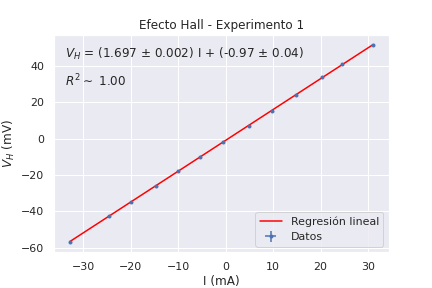
\includegraphics[width=\linewidth]{experimento1}
	\caption{Dependencia de la intensidad con la distancia}
	\label{figure_exp1}
\end{figure}

Como es de esperar obtenemos una dependencia $J \propto \frac{1}{r^2}$, lo cual, si aplicamos logaritmos a nuestros datos deberíamos obtener una dependencia $Ln \left(J\right) \propto -2Ln(r)$, resultados que se muestran en la figura (\ref{figure_exp1_reg}) además de su correspondiente regresión lineal. Vemos que hay una discrepancia entre el valor esperado (-2) y el valor de la pendiente de la regresión ya que la dependencia $J \propto \frac{1}{r^2}$ es para una fuente ideal y sin pérdidas, realidad que no corresponde con nuestro experimento.

\begin{figure}[t]
	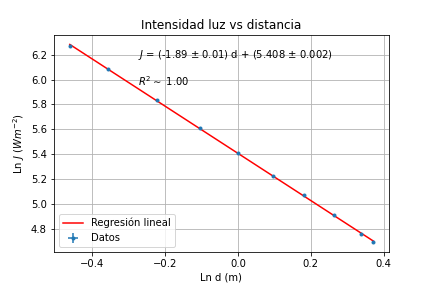
\includegraphics[width=\linewidth]{experimento1_reg}
	\caption{Dependencia del logaritmo intensidad con la distancia}
	\label{figure_exp1_reg}
\end{figure}

Una vez medida la intensidad de luz que llega a nuestra célula pasaremos a estudiar las curvas I-V a varias intensidades de luz. A las distancias de 70, 110 y 150 cm y, haciendo uso de un reostato, variamos poco a poco la resistencia de la carga desde $V=V_{OC}$ (o $I = I_{SC}$) para medir valores de intensidad y voltaje. Los resultados se muestran en la figura (\ref{figure_exp2}), donde además de han selañado los puntos $V_{OC}$, $I_{SC}$ y $P_{max}$. Con estos datos podemos calcular ciertos parámetros de interés como son el factor de llenado (factor de forma) y la eficiencia de la célula solar.

\begin{figure}[t]
	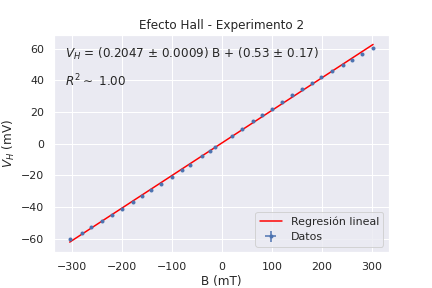
\includegraphics[width=\linewidth]{experimento2}
	\caption{Dependencia de la corriente de cortocircuito con la tensión de circuito abierto para distancias de 70, 110 y 150 cm.}
	\label{figure_exp2}
\end{figure}

En la tabla (\ref{table_exp2}) vemos como la intensidad luminosa que llega a la célula $I_{SC}$ y $V_{OC}$ son inversamente proporcionales a la distancia en la que se encuentra la célula. La potencia máxima alcanza un máximo cuando la célula se encuentra alrededor de los 110cm mientras que la resistencia aumenta a medida que también aumenta la distancia. El factor de forma FF se mantiene constante al ser un parámetro característico del dispositivo mientras que la eficiencia de la célula, cuyo valor bastante bajo ronda el 4\%, también disminuye a medida que la célula se encuentra más alejada del foco de luz.

\begin{table}[t]
	\centering
	\begin{adjustwidth}{-2cm}{}
	\begin{tabular}{cccc}
		\toprule
		\multicolumn{1}{c}{} & \multicolumn{3}{c}{Distancia (cm)} \\
		\cmidrule(r){2-4}
		& $70.0 \pm 0.1$    & $110.0 \pm 0.1$    & $150.0 \pm 0.1$ \\
		\midrule
		J ($Wm^2$) & $439.8 \pm 0.4$    & $186.4 \pm 0.4$    & $110.2 \pm 0.4$ \\
		$I_{SC} (\cdot 10^{-3}A)$ & $67.1 \pm 0.1$    & $29.8 \pm 0.1$    & $15.8 \pm 0.1$ \\
		$V_{OC} (\cdot 10^{-2}V)$ & $220.0 \pm 0.1$    & $201.0 \pm 0.1$    & $192.0 \pm 0.1$ \\
		$P_{max} (mW)$ & $107.4 \pm 0.2$    & $422.40 \pm 0.19$    & $219.99 \pm 0.17$ \\
		R ($\Omega$) & $30.66 \pm 0.07$    & $60.6 \pm 0.2$    & $121.1 \pm 0.9$ \\
		FF $(\cdot 10^{-2})$ & $72.8 \pm 0.4$    & $70.5 \pm 0.8$    & $72.52 \pm 1.5$ \\
		$\eta (\cdot 10^{-3})$ & $48.96 \pm 0.15$    & $45.3 \pm 0.3$    & $39.9 \pm 0.5$ \\
		\bottomrule
	\end{tabular}
	\caption{Resultados curva característica I-V}
	\label{table_exp2}
\end{adjustwidth}
\end{table}

Manteniendo el montaje experimental medimos directamente $I_{SC}$ y $V_{OC}$ para determinar la dependencia frente a la intensidad de luz. Los resultados se visualizan en la figura (\ref{figure_exp3_voc}) donde se presenta la dependencia $V_{OC}$ frente a la intensidad de luz y en la figura (\ref{figure_exp3_reg}) que muestra la dependencia lineal de $I_{SC}$ frente a la intensidad de luz. En concreto tenemos que $I_{SC} = \alpha J$

\begin{figure}[t]
	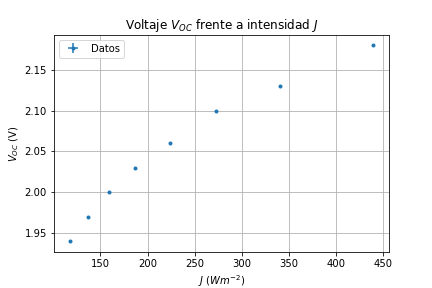
\includegraphics[width=\linewidth]{experimento3_voc}
	\caption{Voltaje $V_{OC}$ frente a intensidad $J$ para distancias}
	\label{figure_exp3_voc}
\end{figure}

\begin{figure}[t]
	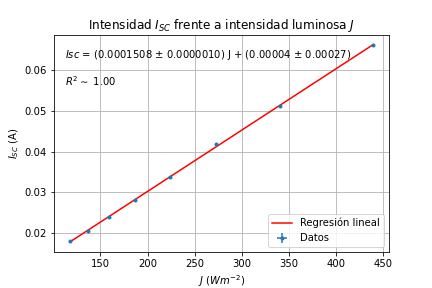
\includegraphics[width=\linewidth]{experimento3_reg}
	\caption{Intensidad $I_{SC}$ frente a intensidad luminosa $J$}
	\label{figure_exp3_reg}
\end{figure}

Para medir el efecto de la temperatura en las curvas características I-V tomaremos datos haciendo dos modificaciones. En primer lugar interpondremos un cristal de vidrio entre el foco de luz y la célula solar y, en segundo lugar, calentaremos directamente la célula de aire gracias a una corriente continua de aire a 60ºC.

Podemos ver en la figura (\ref{figure_exp4}) estos resultados. En primera instancia vemos que la curva I-V para el cristal y el aire caliente permanecen con valores inferiores a la curva I-V en condiciones normales (con la temperatura ambiente de 27ºC). En cuanto a las modificaciones en sí mismas vemos que el valor de $I_{SC}$ para la curva I-V del aire caliente es superior a la curva del cristal, mientras que $V_{OC}$ ocurre al revés. Con lo cual se produce un decaimiento más pronunciado hacia $V_{OC}$ en el caso del aire caliente.

En los datos proporcionados por el fabricante nos dice que $\frac{\Delta V_{OC}}{\Delta T} \sim -8$mV/K, por lo que para cada celda se debería obtener alrededor de -2mV/K (la batería está compuesta de 4 celdas en serie). En nuestro caso obtenemos $\frac{\Delta V_{OC}}{\Delta T} = -4.8 \pm 0.6$mV/K. Las discrepancias en estos valores pueden deberse a las diferencias en las condiciones de laboratorio entre fabricante y nosotros, pues nuestro dispositivo experimental es muy rudimentario y las condiciones de temperatura quizás no sean muy fehacientes. Es posible también que la dependencia con la temperatura en el rango estudiado no sea lineal. Además, tampoco sabemos las condiciones luminosas del fabricante.

\begin{figure}[t]
	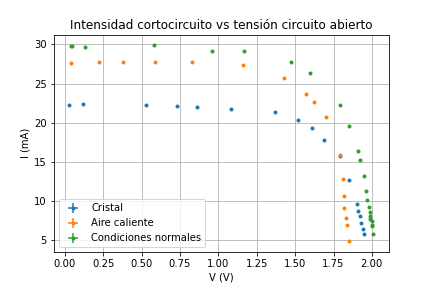
\includegraphics[width=\linewidth]{experimento4}
	\caption{Efecto de la temperatura sobre la corriente de cortocircuito y la tensión de circuito abierto. Distancia de 110cm al foco de luz.}
	\label{figure_exp4}
\end{figure}

Para finalizar representamos los datos I-V y parámetros relevantes de la célula bajo exposición solar en la figura (\ref{figure_exp5}) y la tabla (\ref{table_exp5})

\begin{figure}[t]
	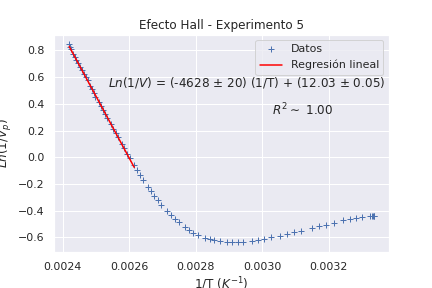
\includegraphics[width=\linewidth]{experimento5}
	\caption{Dependencia de la corriente de cortocircuito con la tensión de circuito abierto bajo exposición solar.}
	\label{figure_exp5}
\end{figure}

\begin{table}[t]
	\centering
	\begin{tabular}{cc}
		\toprule
		\multicolumn{1}{c}{} & \multicolumn{1}{c}{$V_{th}$} \\
		\cmidrule(r){2-2}
		& $25.8 \pm 0.1$mV     \\
		\midrule
		J ($Wm^2$) & $1137.1 \pm 0.4$    \\
		$I_{SC} (\cdot 10^{-3}A)$ & $390.0 \pm 0.1$    \\
		$V_{OC} (\cdot 10^{-2}V)$ & $231.0 \pm 0.1$    \\
		$P_{max} (mW)$ & $661.5 \pm 0.5$    \\
		R $(\Omega \cdot 10^{-2})$ & $540.0 \pm 0.4$    \\
		FF $(\cdot 10^{-2})$ & $73.4 \pm 0.1$    \\
		$\eta (\cdot 10^{-3})$ & $116.4 \pm 0.14$    \\
		\bottomrule
	\end{tabular}
	\caption{Resultados curva característica I-V bajo exposición solar}
	\label{table_exp5}
\end{table}

En este caso podemos ver que la eficiencia de la célula solar es muy superior al foco de luz (junto con los parámetros $I_{SC}$, $V_{OC}$, $P_{max}$), dando casi un valor del 12\%, consecuencia directa de que contamos con una fuente luminosa mucho mayor. Si calculamos el valor de $I_{SC}$ mediante la regresión anterior $I_{SC} = \alpha J$ obtenemos $I_{SC} = 0.1715 \pm 0.0012$A